%
% This is the LaTeX template file for lecture notes for EE 382C/EE 361C.
%
% To familiarize yourself with this template, the body contains
% some examples of its use.  Look them over.  Then you can
% run LaTeX on this file.  After you have LaTeXed this file then
% you can look over the result either by printing it out with
% dvips or using xdvi.
%
% This template is based on the template for Prof. Sinclair's CS 270.

\documentclass[twoside]{article}
\usepackage{amsmath}
\usepackage{graphics}
\usepackage{graphicx}
\usepackage{algorithm}
\usepackage{algpseudocode}
\usepackage{qtree}
\usepackage{pgfplots}
\usepackage{tikz-qtree}
\setlength{\oddsidemargin}{0.25 in}
\setlength{\evensidemargin}{-0.25 in}
\setlength{\topmargin}{-0.6 in}
\setlength{\textwidth}{6.5 in}
\setlength{\textheight}{8.5 in}
\setlength{\headsep}{0.75 in}
\setlength{\parindent}{0 in}
\setlength{\parskip}{0.1 in}

%
% The following commands set up the lecnum (lecture number)
% counter and make various numbering schemes work relative
% to the lecture number.
%
\newcounter{lecnum}
\renewcommand{\thepage}{\thelecnum-\arabic{page}}
\renewcommand{\thesection}{\thelecnum.\arabic{section}}
\renewcommand{\theequation}{\thelecnum.\arabic{equation}}
\renewcommand{\thefigure}{\thelecnum.\arabic{figure}}
\renewcommand{\thetable}{\thelecnum.\arabic{table}}

%
% The following macro is used to generate the header.
%
\newcommand{\lecture}[4]{
   \pagestyle{myheadings}
   \thispagestyle{plain}
   \newpage
   \setcounter{lecnum}{#1}
   \setcounter{page}{1}
   \noindent
   \begin{center}
   \framebox{
      \vbox{\vspace{2mm}
    \hbox to 6.28in { {\bf EE 382V: Parallel Algorithms
                        \hfill Summer 2017} }
       \vspace{4mm}
       \hbox to 6.28in { {\Large \hfill Lecture #1: #2  \hfill} }
       \vspace{2mm}
       \hbox to 6.28in { {\it Lecturer: #3 \hfill Scribe: #4} }
      \vspace{2mm}}
   }
   \end{center}
   \markboth{Lecture #1: #2}{Lecture #1: #2}
   %{\bf Disclaimer}: {\it These notes have not been subjected to the
   %usual scrutiny reserved for formal publications.  They may be distributed
   %outside this class only with the permission of the Instructor.}
   \vspace*{4mm}
}

%
% Convention for citations is authors' initials followed by the year.
% For example, to cite a paper by Leighton and Maggs you would type
% \cite{LM89}, and to cite a paper by Strassen you would type \cite{S69}.
% (To avoid bibliography problems, for now we redefine the \cite command.)
% Also commands that create a suitable format for the reference list.
\renewcommand{\cite}[1]{[#1]}
\def\beginrefs{\begin{list}%
        {[\arabic{equation}]}{\usecounter{equation}
         \setlength{\leftmargin}{2.0truecm}\setlength{\labelsep}{0.4truecm}%
         \setlength{\labelwidth}{1.6truecm}}}
\def\endrefs{\end{list}}
\def\bibentry#1{\item[\hbox{[#1]}]}

%Use this command for a figure; it puts a figure in wherever you want it.
%usage: \fig{NUMBER}{SPACE-IN-INCHES}{CAPTION}
\newcommand{\fig}[3]{
			\vspace{#2}
			\begin{center}
			Figure \thelecnum.#1:~#3
			\end{center}
	}
% Use these for theorems, lemmas, proofs, etc.
\newtheorem{theorem}{Theorem}[lecnum]
\newtheorem{lemma}[theorem]{Lemma}
\newtheorem{proposition}[theorem]{Proposition}
\newtheorem{claim}[theorem]{Claim}
\newtheorem{corollary}[theorem]{Corollary}
\newtheorem{definition}[theorem]{Definition}
\newenvironment{proof}{{\bf Proof:}}{\hfill\rule{2mm}{2mm}}

% **** IF YOU WANT TO DEFINE ADDITIONAL MACROS FOR YOURSELF, PUT THEM HERE:

\begin{document}
%FILL IN THE RIGHT INFO.
%\lecture{**LECTURE-NUMBER**}{**DATE**}{**LECTURER**}{**SCRIBE**}
\lecture{1}{June 9}{Vijay Garg}{Hector Jesus Acosta Garcia}
%\footnotetext{These notes are partially based on those of Nigel Mansell.}

% **** YOUR NOTES GO HERE:

% Some general latex examples and examples making use of the
% macros follow.  
%**** IN GENERAL, BE BRIEF. LONG SCRIBE NOTES, NO MATTER HOW WELL WRITTEN,
%**** ARE NEVER READ BY ANYBODY.
\section{Memory Hierarchy}


Memory Hierarchy can be used to discuss performance issues in computer programs.
Throughout this course, an emphasis is made on the time and work complexity of
algorithms, however there are other factors that can affect real world performance of
processes executing different algorithms. After an algorithm is implemented,
it is important to verify cache behavior and other lower level.

From faster to slower the memory hierarchy follows:
\begin{itemize}
	\item Processor Registers
	\item Processor caches (L1, L2, L3, \ldots)
	\item Main memory
	\item Disk
\end{itemize}

Accessing data on a lower level in the above hierarchy orders of magnitude of slowdown.

\section{PRAM}
PRAM is the parallel analogous to RAM for parallel algorithm. It is
assumed to be shared by more than one processor, and at any point in
time a processor can read or write to any memory location.

\begin{figure}[!ht]
\centering
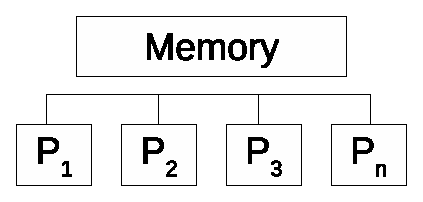
\includegraphics[scale=0.6]{memory.eps}
\caption{A PRAM representation}
\end{figure}


All processors work in lock-step. Occasionally, a "BARRIER" instruction
is needed, this is similar tu syncThreads() in CUDA.

In PRAM, the following are valid Read/write conflict resolution strategies:

\begin{tabular}{|l|l|p{8cm}|}
	\hline
	EREW & Exclusive Reads Exclusive Writes & Most flexible. Every memory location can be read or written to by only one processor at the time. Algorithms designed for this conflict strategy, work for all conflict strategies. \\ \hline
	CREW & Concurrent Reads Exclusive Writes & Closest to reality. \\ \hline
	ERCW & Exclusive Reads Concurrent Writes & Not interesting. \\  \hline
	CRCW & Concurrent Reads Concurrent Writes & Fastest model. \\ \hline
\end{tabular}

For concurrent writes, PRAM can be further defined as:
\begin{itemize}
	\item Arbitrary: Choose arbitrarily when two concurrent writes are performed to the same memory location
	\item Common: All processors must write the same value.
	\item Priority: Processor id is used to resolve conflicts.
\end{itemize}

\section{Network}

In a parallel computing system, there are several types of Network topologies that
can be used.

\begin{itemize}
 \item Mesh: data is transmited at 1 unit per hop
 \item Torus: Mesh with wraparound link at the edges
 \item Completely connected: Not efficient or scalable.
\end{itemize}

\subsection{Hypercube}

In a hypercube with $n ^d$ nodes, the maximum distance between two nodes is
$ d $.

If each node can be labeled by a $d$-bit string, two nodes are connected if they differ in exactly
$1$ bit.

\begin{figure}[!ht]
\centering
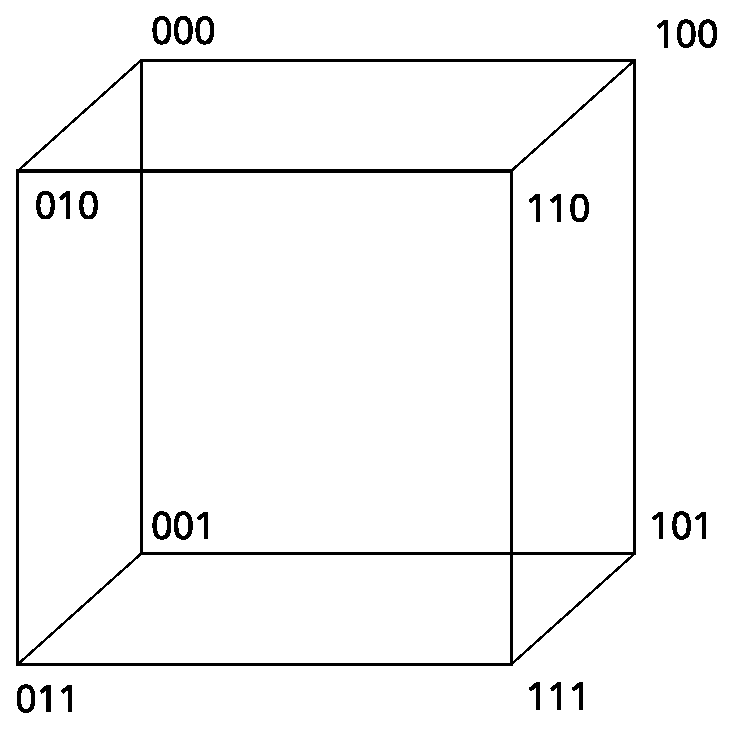
\includegraphics[scale=0.3]{cube.eps}
\caption{An 8 node hypercube with $d = 3 $}
\end{figure}

\section{Scalability}
\subsection{Strong Scalability}
As the number of cores increases, the time taken to solve the same problem decreases.

\subsection{Weak Scalability}
For the same problem $ problemSize / numberOfCores = Constant $

\subsection{Amadahl's Law}
Amadahl's law is used to calculate the maximum speedup possible by improving the parallel portion
of an algorithm. Assume a program can be divided into sequential part $s$ and non-sequential part
$ 1 - s $, and $n$ is the number of processors. Then, the speedup can be given by:

\begin{align*}
 speedup &= \frac{T_{seq}}{T_{parallel}}\\
 T_{parallel} &\geq s(T_{seq}) + \frac{(1 - s) T_{seq}}{n} \\
 T_{parallel} &\geq (s + \frac{1 -s }{n}) T_{seq} \\
 \frac{T_{seq}}{T_{parallel}} &\leq \frac{1}{s + \frac{1 - s}{n}}
\end{align*}


\subsection{Gustafson's Law}

Gustafson argues that the problem size is not constant and if the parallel portion of a program is improved,
the problem size may also be increased, while solving the problem in the same time.

\section{Programming Languages}

In class, we briefly went over the following example programs (found in the course's github page).

\begin{itemize}
 \item FooBar.java
 \item Fibonacci1.java
 \item Fibonacci2.java
 \item Fibonacci3.java
\end{itemize}


\end{document}





